%=======================================================================
%
% ------------------------------------------------------------------------
% ------------------------------------------------------------------------
% abnTeX2: Modelo de Trabalho Academico  em conformidade com 
% ABNT NBR 14724:2011: Informacao e documentacao - Trabalhos academicos
% ------------------------------------------------------------------------
%Customização Unoesc
% ------------------------------------------------------------------------
% Autor:  Jonas Alessi(alessi.jonas@gmail.com
% Versão: 10 de Julho 2013.
% Edição: TexStudio
% Codificação: UTF-8
% LaTeX:  abnTeX2
%
%=======================================================================

\documentclass[
	% -- opções da classe memoir --
	12pt,				% tamanho da fonte	
	oneside,          % não imprimir em verso e anverso, oposto do twoside 
	a4paper,			% tamanho do papel. 
	% -- opções da classe abntex2 --
	chapter=TITLE,		% títulos de capítulos convertidos em letras maiúsculas
	section=TITLE,		% títulos de seções convertidos em letras maiúsculas
	subsection=TITLE,	% títulos de subseções convertidos em letras maiúsculas
	%subsubsection=TITLE,% títulos de subsubseções convertidos em letras maiúsculas
	% -- opções do pacote babel --
	english,			% idioma adicional para hifenização
	brazil			% o último idioma é o principal do documento
	,sumario=tradicional,
	]{abntex2-unoesc}


% ---
% Pacotes fundamentais 
% ---
\usepackage{cmap}				% Mapear caracteres especiais no PDF
\usepackage{times}			    % Usa a fonte Latin Modern			
\usepackage[T1]{fontenc}		% Selecao de codigos de fonte.
\usepackage[utf8]{inputenc}		% Codificacao do documento (conversão automática dos acentos)
\usepackage{lastpage}			% Usado pela Ficha catalográfica
\usepackage{indentfirst}		% Indenta o primeiro parágrafo de cada seção.
\usepackage{color}				% Controle das cores
\usepackage{graphicx}			% Inclusão de gráficos
\usepackage{amsfonts}			% Símbolos
\usepackage{amsmath}
\usepackage{caption}
\usepackage{enumitem}
\usepackage{pdfpages}
\usepackage{multirow}
\usepackage{multicol}

\setitemize[0]{itemindent=0.4cm,itemsep=0pt}
\setenumerate[0]{itemindent=0.5cm,itemsep=0pt}
%------
% ---
% Pacotes de citações
% ---
\usepackage[brazilian,hyperpageref]{backref}	 					  % Paginas com as citações na bibl

%Referência
\usepackage[alf, 	
			 		abnt-emphasize=bf,
				    abnt-url-package=none,
				    abnt-repeated-title-omit=yes,
				    abnt-full-initials=yes,                                        %yes nome por extenso, no apenas iniciais
					abnt-etal-list=3												%abreviar com mais de 3 autores
]{abntex2/abntex2cite}				 	    									    % Citações padrão ABNT
\usepackage{lipsum}							   								       % para geração de dummy text

%\captionsetup[table]{justification=raggedright}
% Configurações de aparência do PDF final
% alterando o aspecto da cor azul
\definecolor{blue}{RGB}{41,5,195}

% --- 
% Espaçamentos entre linhas e parágrafos 
% --- 
% O tamanho do parágrafo é dado por:
\setlength{\parindent}{1.25cm}
\linespread{1.5}

%Espaçamento depois dos títulos
\setlength{\afterchapskip}{\baselineskip}
% %\setlength{\afterchapskip}{\lineskip}

% Controle do espaçamento entre um parágrafo e outro:
\setlength{\parskip}{0cm}  % tente também \onelineskip

\hangcaption
\captionstyle[\raggedright]{}

%Estava mostrando nas referencias quais paginas estavam sendo referenciadas
\renewcommand{\backref}{}
\renewcommand*{\backrefalt}[4]{}

%Reduzir a fonte do caption
\captionnamefont{\centering\ABNTEXfontereduzida}
\captiontitlefont{\centering\ABNTEXfontereduzida}
%Ajuste nas listas de tabela, ilustrações e quadros
\setlength\cftbeforechapterskip{0pt}
% ---
% compila o indice
% ---
\makeindex
% ---

%----Include da capa é fora do documento 
% ---
% Informações de dados para CAPA e FOLHA DE ROSTO
% ---
\titulo{ESTÁGIO SUPERVISIONADO NA EMPRESA...}
\autor{NOME DO ACADÊMICO}
\local{JOAÇABA}
\data{ANO}
\orientador[ORIENTADOR:]{Nome do Orientador}
%\coorientador{Coorientador 2}
\supervisor[SUPERVISOR:]{Nome do Supervisor de estágio}  % no caso de ser estágio
\instituicao{UNIVERSIDADE DO OESTE DE SANTA CATARINA}
\tipotrabalho{Estágio Supervisionado}
% O preambulo deve conter o tipo do trabalho, o objetivo, 
% o nome da instituição e a área de concentração 
\preambulo{Relatório de estágio supervisionado apresentado ao Curso de Engenharia de Computação, Área de Ciências Exatas e Tecnológicas da Universidade do Oeste de Santa Catarina como requisito parcial à obtenção do grau de bacharel em Engenharia de Computação.}
% ---

%---

\begin{document}
% Retira espaço extra obsoleto entre as frases.
\frenchspacing 

% ----------------------------------------------------------
% ELEMENTOS PRÉ-TEXTUAIS
% ----------------------------------------------------------

%--- CAPA ----
\imprimircapa

% --- FOLHA DE ROSTO
\imprimirfolhaderosto
% Na versão final inclua a ficha catalográfica que deve ser solicitada na biblioteca
% \imprimirfolhaderosto
%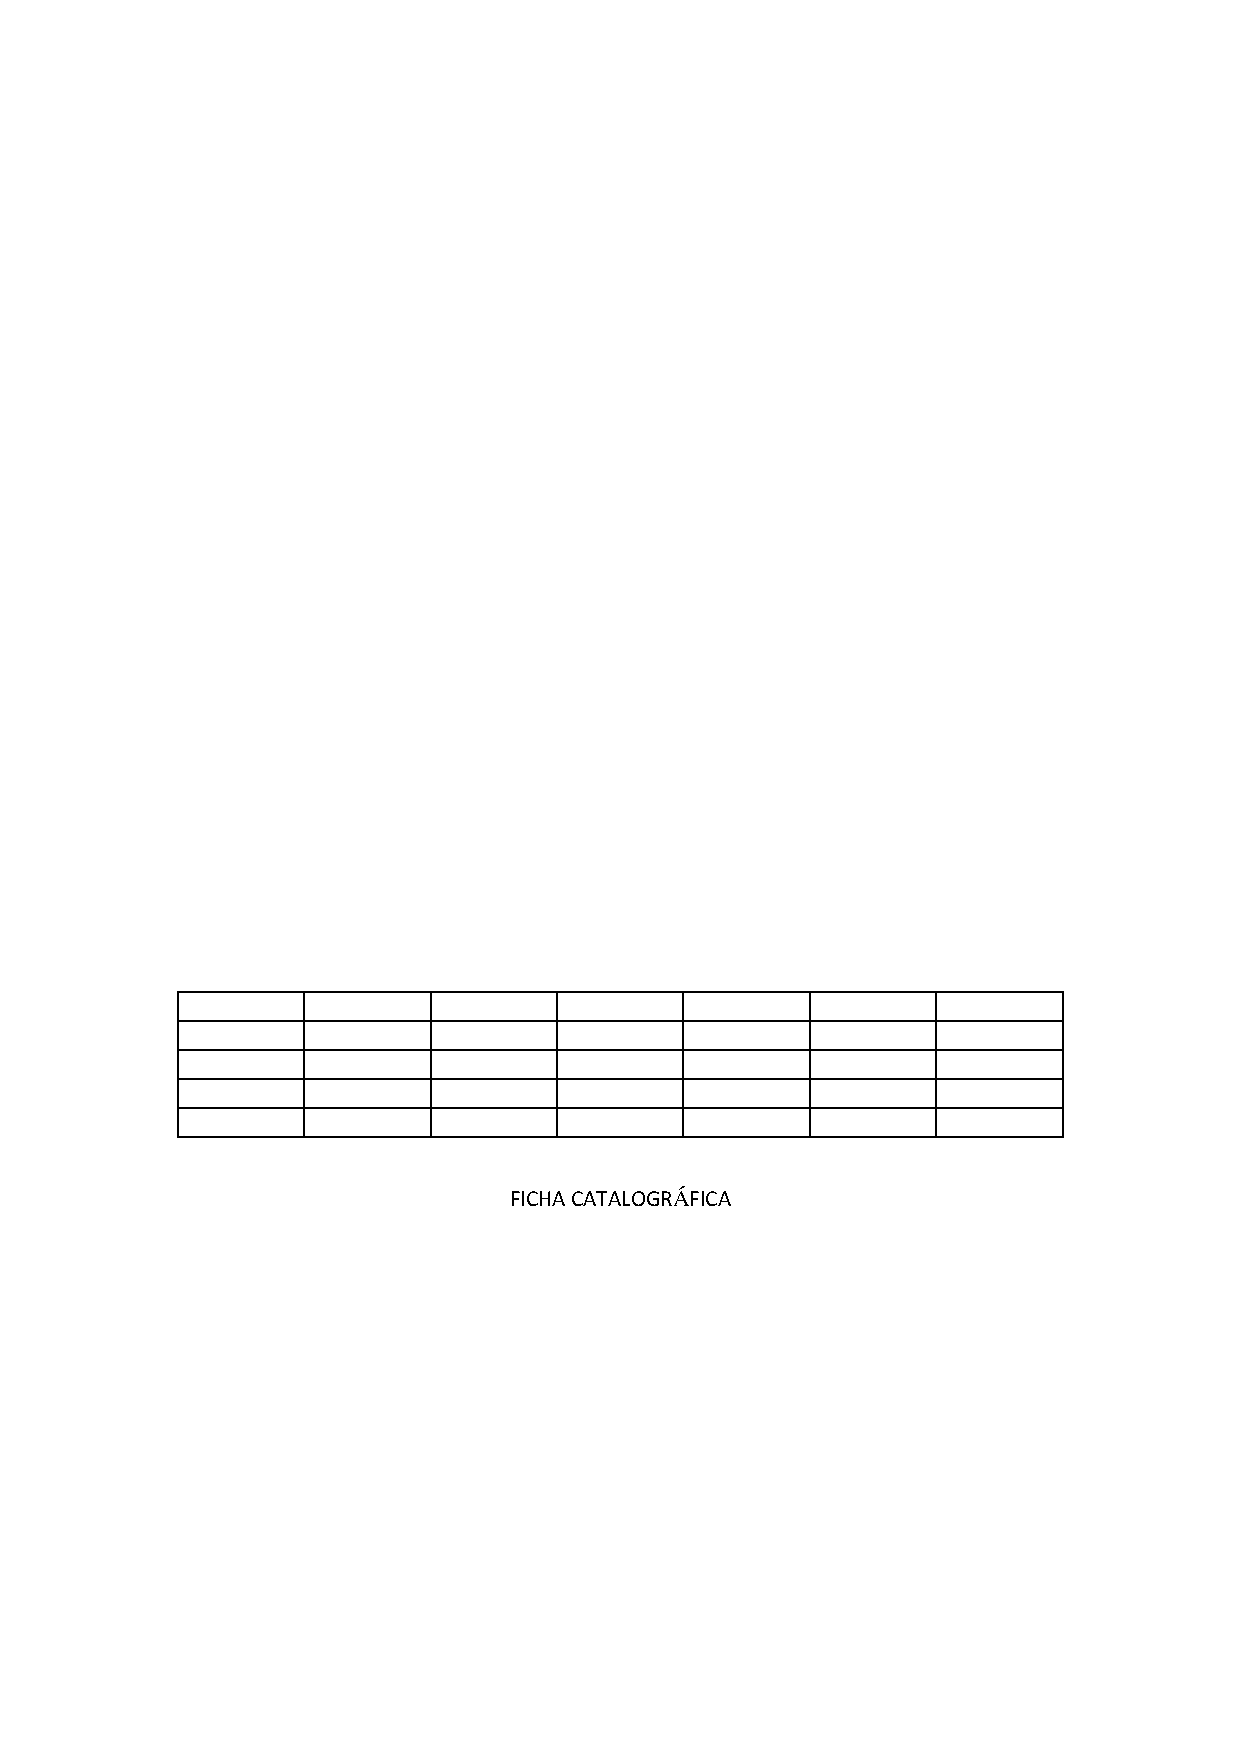
\includepdf{pretextuais/ficha_catalografica}

% Inserir FOLHA DE APROVAÇÃO
% NA VERSÃO FINAL
% retirar a folha de aprovação e incluir a assinada digitalizada em pdf
%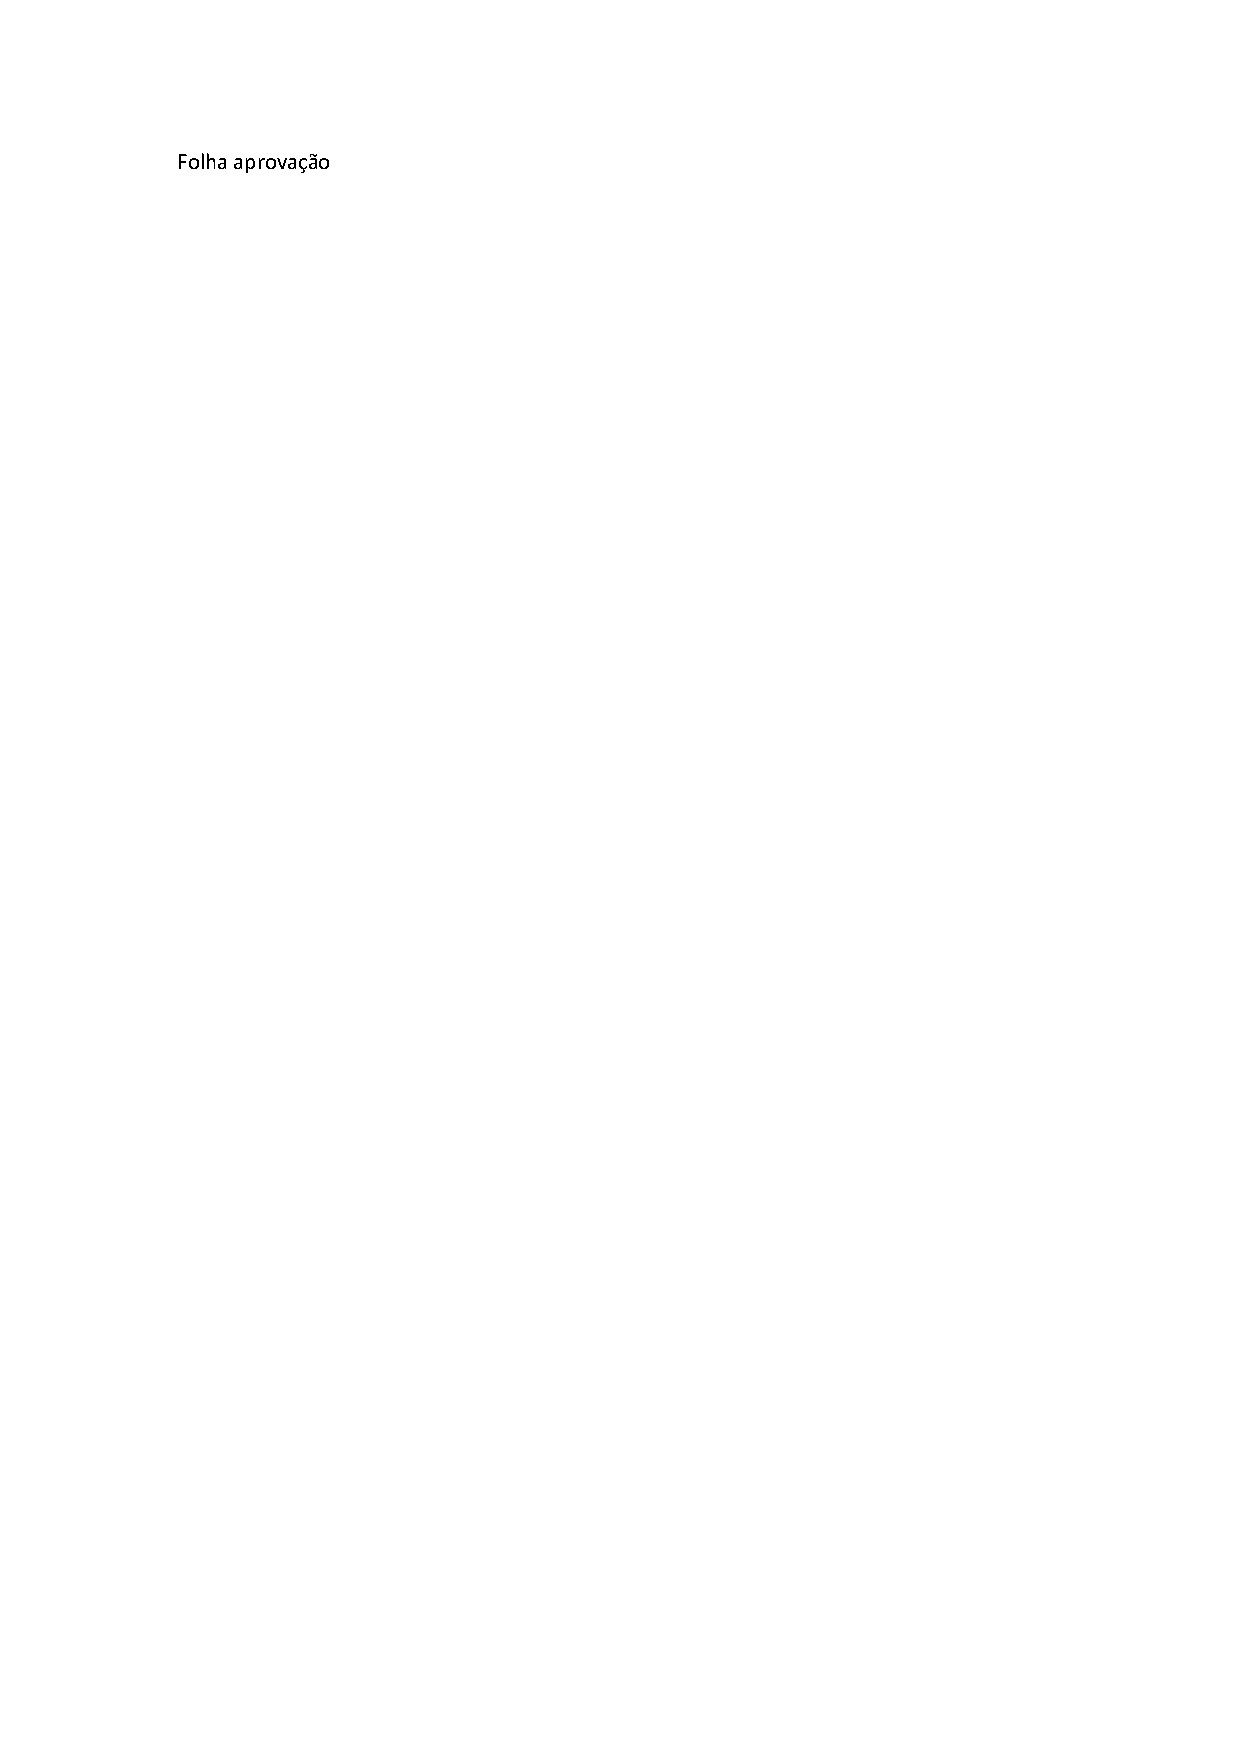
\includepdf{pretextuais/folha}
\begin{folhadeaprovacao}

  \begin{center}
  \vspace*{-1.2cm}
    {\large\imprimirautor}

    \vspace*{\fill}
    {\large\imprimirtitulo}
    \vspace*{\fill}
    
    \hspace{.45\textwidth}
    \begin{minipage}{.5\textwidth}
        \imprimirpreambulo
    \end{minipage}%
    \vspace*{\fill}
   \end{center}
    

  

\vspace{1cm}

  \begin{center}
  	BANCA EXAMINADORA
  \end{center}
   \assinatura{\imprimirorientador \\ 
   					   Universidade do Oeste de Santa Catarina
   					    
   } 
   \assinatura{Professor \\ 
   					   Universidade do Oeste de Santa Catarina
   					    
   }
    \assinatura{Professor \\ 
   					   Universidade do Oeste de Santa Catarina
   					   
    }
      
%   \begin{center}
    \vspace*{3cm}
%    {\large\imprimirlocal}
%    \par
%    {\textbf{\large\imprimirdata}}
%    \vspace*{1cm}
%  \end{center}
  
\end{folhadeaprovacao}

% DEDICATÓRIA
\begin{dedicatoria}
 \vspace*{\fill}
 \noindent
  \raggedleft
 \begin{minipage}{.54\textwidth}
   Faça aqui sua dedicatória. Faça aqui sua dedicatória. Faça aqui sua dedicatória. Faça aqui sua dedicatória. Faça aqui sua dedicatória.
   \end{minipage}
\end{dedicatoria}


% AGRADECIMENTO
\begin{agradecimentos}

\textit{Agradeça aqui! Agradeça aqui! Agradeça aqui! Agradeça aqui! Agradeça aqui! Agradeça aqui!}




\end{agradecimentos}

%EPÍGRAFE
\begin{epigrafe}
    \vspace*{\fill}
	\begin{flushright}
		``Com grandes poderes vêm grandes\\
		responsabilidades''\\
		(Benjamin Parker)
	\end{flushright}
\end{epigrafe}

% RESUMO

% resumo em português
\begin{resumo}
\noindent
\lipsum[1-1] %Aqui vai o resumo

 \vspace{0.2cm}
    
 
 Palavras-chave: Latex. Abntex. Editoração de texto.
\end{resumo}

% resumo em inglês
\begin{resumo}[Abstract]	
 	\begin{otherlanguage*}{english}
 	\noindent 
	\textit{
	\lipsum[1-1]  % Aqui vai o abstract
	} 
   \vspace{0.2cm}
 
   
    Key-words: Latex. Abntex. Text editoration.	
 	\end{otherlanguage*}
\end{resumo}

% lista de ilustrações
\pdfbookmark[0]{\listfigurename}{lof}
\listoffigures*
\cleardoublepage
% ---

% lista de quadros
% --- 
%PRECISO VER COMO FAZER O CONTROLE DE QUANDO TIVER MENOS Q 10 VAI PARA LISTA DE ILUSTRAÇÕES
\pdfbookmark[0]{\listofquadrosname}{loq}
\listofquadros*
\cleardoublepage
% ---

% LISTA DE TABELAS
\pdfbookmark[0]{\listtablename}{lot}
\listoftables*
\cleardoublepage  %-- força proxima pagina

% ---
% inserir lista de abreviaturas e siglas
% ---
\begin{siglas}
  \item[ABNT] Associação Brasileira de Normas Técnicas
  \item[CNPq] Conselho Nacional de Desenvolvimento Científico e Tecnológico
  \item[IBGE] Instituto Brasileiro de Geografia e Estatística
  \item[LCD] \textit{Liquid Crystal Dysplay} (Display de cristal líquido)
\end{siglas}
% ---

% ---
% inserir lista de símbolos
% ---
\begin{simbolos}
  \item[$ \Gamma $] Descrever o que o símbolo representa em seu trabalho. Exemplo abaixo.
  \item[$ \omega $] Frequência angular [rad/s].
  \item[$ \zeta $] Coeficiente de amortecimento.

\end{simbolos}
% ---

% SUMARIO
\pdfbookmark[0]{\contentsname}{toc}
\tableofcontents*
\cleardoublepage

% ------------------------------------------------------
% ELEMENTOS TEXTUAIS
% ------------------------------------------------------
\textual
% INTRODUÇÃO
% ----------------------------------------------------------
% Introdução
%Ex: \chapter{TÍTULO A SER IMPRESSO NO CORPO DO TEXTO}{Título no cabeçalho}{Título no Sumario}
% ----------------------------------------------------------
\chapter{INTRODUÇÃO} % se usar o \chapter* ele não vai colocar no sumario
%\addcontentsline{toc}{chapter}{Introdução} inclui manualmente no sumario sem numeração
\lipsum[1-1]

\section{DESCRIÇÃO DO PROBLEMA}
\lipsum[1-1]

\section{JUSTIFICATIVA}
O n$^\circ$ Nam dui ligulaquet magna, vitae ornare odio metus a mi. Morbi ac orci et nisl hendrerit mollis. Suspendisse ut massa suspendisse ut massa a suspendisse ut massa a suspendisse ut massa.Nam dui ligulaquet magna, vitae ornare odio metus a mi. Morbi ac orci et nisl hendrerit mollis. Suspendisse ut massa suspendisse ut massa a suspendisse ut massa a suspendisse ut massa.

\section{OBJETIVOS}

\subsection{Objetivo geral}
Nam dui ligulaquet magna, vitae ornare odio metus a mi. Morbi ac orci et nisl hendrerit mollis. Suspendisse ut massa suspendisse ut massa a suspendisse ut massa a suspendisse ut massa.

\subsection{Objetivos específicos}
Desdobramento do objetivo geral. 
 \begin{itemize}
	\item Item 1
	\item Item 2
	\item Item 3
	\item texto
\end{itemize}

 \section{ORGANIZAÇÃO DO TRABALHO}
 \lipsum[1-1]

%FUNDAMENTAÇÃO TEÓRICA
\chapter{FUNDAMENTAÇÃO TEÓRICA}
\label{cap:fundamentacao}


Apresentar estudos que contemple a temática abordada. Respeitar a autoria,
nas citações diretas e indiretas. Evitar parágrafos muito longos. Evitar seções e
subseções muito curtas. Conforme \ref{eq:1} ...

\begin{equation}
\label{eq:2}
x = \frac{{ - b \pm \sqrt {{b^2} - 4\,ac} }}{{2a}}
\end{equation}

\begin{equation}
\label{eq:1}
\left[ {\begin{array}{*{20}{c}}
	1&0&0\\
	0&1&0\\
	0&0&1
	\end{array}} \right] = I
\end{equation}



A parcela $ \frac{-b}{2a}$ é ...

\section{Exemplo de Seção}
\label{sec:apresentacao}


\subsection{Exemplo subSeção}

\subsubsection{Exemplo subsubsection}

% FALTA AJUSTAR \subsubsubsection{Exemplo subsubsubsection}

%DESENVOLVIMENTO
\chapter{DESENVOLVIMENTO}

Nam dui ligula, fringilla a, euismod sodales, sollicitudin vel, wisi. Morbi auctor lorem non justo. Nam lacus libero, pretium at, lobortis vitae, ultricies et, tellus. Donec aliquet, tortor sed accumsan bibendum, erant montes, nascetur ridiculus mus. Aliquam tincidunt urna. Nulla ullamcorper vestibulum turpis. Pellentesque cursus luctus mauris \cite{LUCKMANN2008,fitzgerald2014}.

Nam dui ligulna, vitae ornare odio metus a mi. Morbi ac orci et nisl hendrerit mollis. Suspendisse ut massa. Cras nec ante. Pellentesque a nulla. Cum sociis natoque penatibus et magnis dis parturient montes, nascetur ridiculus mus. Aliquam tincidunt urna. Nulla ullamcorper vestibulum turpis. Pellentesque cursus luctus mauris \cite{Telles1984}.

Nao metus a mi. Morbi ac orci et nisl hendrerit mollis. Suspendisse ut massa. Cras nec ante. Pellentesque a nulla. Cum sociis natoque penatibus et magnis dis parturient montes, nascetur ridiculus mus. Aliquam tincidunt urna. Nulla ullamcorper vestibulum turpis. Pellentesque cursus luctus mauris \cite{abntex2-wiki-como-customizar}.

Nam duina, vitae ornare odio metus a mi. Morbi ac orci et nisl hendrerit mollis. Suspendisse ut massa. Cras nec ante. Pellentesque a nulla. Cum sociis natoque penatibus et magnis dis parturient montes, nascetur ridiculus mus. Aliquam tincidunt urna. Nulla ullamcorper vestibulum turpis. Pellentesque cursus luctus mauris \cite{abntex2modelo}.

Nam dui ligulaquet magna, vitae ornare odio metus a mi. Morbi ac orci et nisl hendrerit mollis. Suspendisse ut massa. Cras nec ante. Pellentesque a nulla. Cum sociis natoque penatibus et magnis dis parturient montes, nascetur ridiculus mus \textsuperscript{\textregistered}. Aliquam tincidunt urna. Nulla ullamcorper vestibulum turpis. Pellentesque cursus luctus mauris \cite{memoir}.
\section{SÍMBOLOS}
Marca registrada\textsuperscript{\textregistered}:
	\begin{verbatim}
	\textsuperscript{\textregistered}
	\end{verbatim}

\copyright Copyrigth:
	\begin{verbatim}
	\copyright
	\end{verbatim}
	
	\texttrademark Trademark:
		\begin{verbatim}
		\texttrademark
		\end{verbatim}
\section{SEÇÃO}

 Todas as \textbf{tabelas} e \textbf{figuras} deverão usar a macro \textbf{IBGEtab}, a qual faz o alinhamento a esquerda da legenda e fonte.
 \begin{verbatim}
 \IBGEtab{
 	\caption{xxxx} 
 	\label{xx:xxxx}
 } {
 	tabela ou figura
 } {
 	\fonte{xxxx}
 }
 \end{verbatim} 
 
 Para alinhar a esquerda as \textbf{figuras} ou \textbf{fabelas} deverá ser usada a macro  \textbf{leftable}. Exemplo:
 \begin{verbatim}
 \begin{table}[htb]
  \leftable
  ......
  ....
  \end{table}
 \end{verbatim}
 
 Para criar borda nas \textbf{figuras} poderá ser usada a macro \textbf{borda}. Exemplo:
 \begin{verbatim}
 	\borda{
  		\includegraphics[scale=0.4]{figuras/......}
     }
 \end{verbatim}
\subsection{Subseção de desenvolvimento}

\lipsum[1-1]


\subsection{Tabela}

Uma grande dica aqui é a utilização do site \textbf{www.tablesgenerator.com} para geração de tabelas.

\begin{table}[!htpb]
	\centering
	\caption{Título da tabela}
	\label{my-label}
	\begin{tabular}{lcc}
		& \multicolumn{1}{l}{Coluna 2} & \multicolumn{1}{l}{Coluna 2} \\ \hline
		Linha 1 & a                            & b                            \\ \hline
		Linha2  & c                            & d                           
	\end{tabular}


\fonte{\citeonline{livro-unoesc}.}
%  \nota{Exemplo de nota}
% \nota[Anotações]{Exemplo nota personalizada}
\end{table}
   






\lipsum[1-1]


\subsection{Imagens}


 \begin{figure}[!htpb]
 \centering
 	\caption{Motor de indução trifásico}
 	\label{fig:Motores}
 	\borda{\includegraphics[scale=0.8]{figuras/motores}}
 	\fonte{\cite{NR10}.}
 \end{figure}

% ----------------- Quadro ------------- %
%O Quadro \ref{fig:ranking} foi criado utilizando o ambiente "quadro".
\begin{quadro}[!htpb]
 \centering
	\caption{Ranking de linguagens de programação - Fev/2009}
	\label{fig:ranking}
 	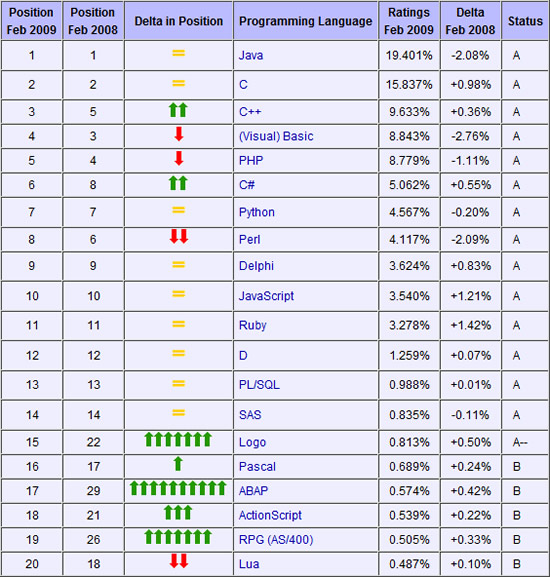
\includegraphics[width=\textwidth]{figuras/ranking}
    \fonte{o autor.}
\end{quadro}

% ----------------- Gráfico ------------- %
%O Gráfico \ref{fig:grafico2} foi criado utilizando o ambiente "grafico".
\begin{grafico}[!htpb]
 \centering
	\caption{Exemplo de gráfico}
	\label{graf:grafico2}
 	\borda{
 		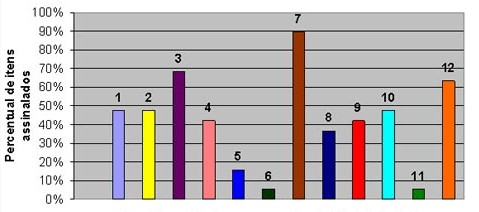
\includegraphics[scale=0.4]{figuras/grafico}
    }
    \fonte{o autor.}
\end{grafico}



% ----------------- Fotografia ------------- %
%A Fotografia \ref{fig:grafico3} foi criado utilizando o ambiente "fotografia".
\begin{fotografia}[!htpb]
 \centering
	\caption{Exemplo de fotografia}
	\label{fot:grafico3}
 	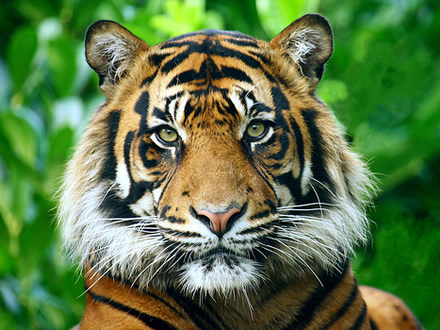
\includegraphics[width=\textwidth]{figuras/fotografia}
    \fonte{o autor.}
\end{fotografia}

% ----------------- Fluxograma ------------- %
%O Fluxograma \ref{fig:grafico4} foi criado utilizando o ambiente "fluxograma".
\begin{fluxograma}[!htpb]
 \centering
	\caption{Exemplo de fluxograma}
	\label{flux:grafico4}
	\borda{
 		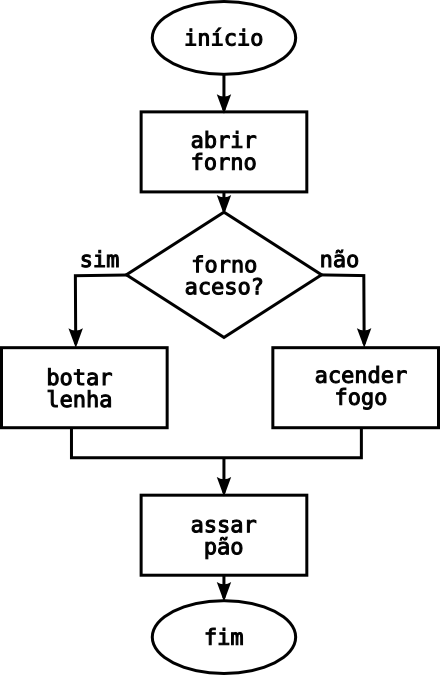
\includegraphics[scale=0.5]{figuras/fluxograma}
    }
    \fonte{o autor.}
\end{fluxograma}



% ----------------- Organograma ------------- %
%O Organograma \ref{fig:grafico5} foi criado utilizando o ambiente "orgonograma".
\begin{organograma}[!htpb]
 \centering
	\caption{Exemplo de organograma}
	\label{orga:grafico5}
	\borda{
 	  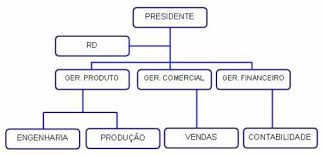
\includegraphics[scale=0.5]{figuras/organograma}
    }
    \fonte{o autor.}
\end{organograma}
% ----------------- Diagrama ------------- %
%O Diagrama \ref{fig:grafico6} foi criado utilizando o ambiente "diagrama".
\begin{diagrama}[!htpb]
 \centering
	\caption{Exemplo de diagrama}
	\label{diag:grafico6}
	\borda{
 	 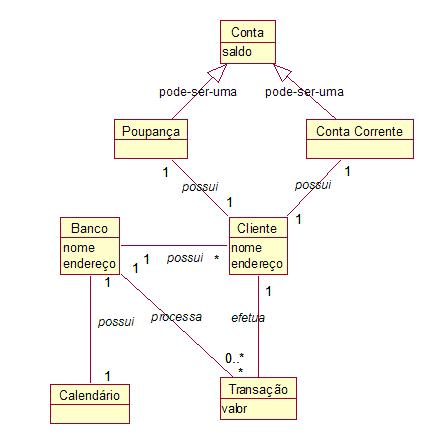
\includegraphics[scale=0.3]{figuras/diagrama}
    }
    \fonte{o autor.}
\end{diagrama}

% ----------------- Mapa ------------- %
%O Mapa \ref{fig:grafico7} foi criado utilizando o ambiente "mapa".
\begin{mapa}[!htpb]
 \centering
	\caption{Exemplo de mapa}
	\label{map:grafico7}
 	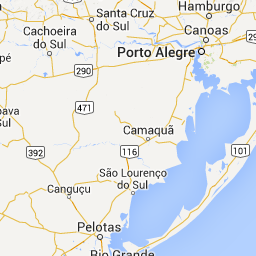
\includegraphics[scale=0.5]{figuras/mapa}
    \fonte{o autor.}
\end{mapa}

% ----------------- Esquema ------------- %
%O Esquema \ref{fig:grafico10} foi criado utilizando o ambiente "esquema".
\begin{esquema}[!htpb]
 \centering
	\caption{Exemplo de esquema}
	\label{esq:grafico10}
	\borda{
 		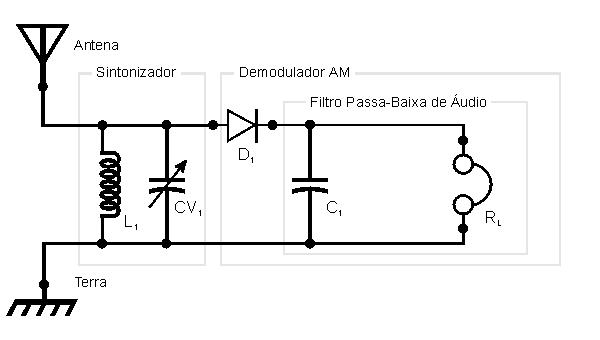
\includegraphics[scale=0.3]{figuras/esquema}
    }
    \fonte{o autor.}
\end{esquema}

% ----------------- Desenho ------------- %
%O Desenho \ref{fig:grafico9} foi criado utilizando o ambiente "desenho".
\begin{desenho}[!htpb]
 \centering
	\caption{Exemplo de desenho}
	\label{des:grafico9}
	\borda{
 		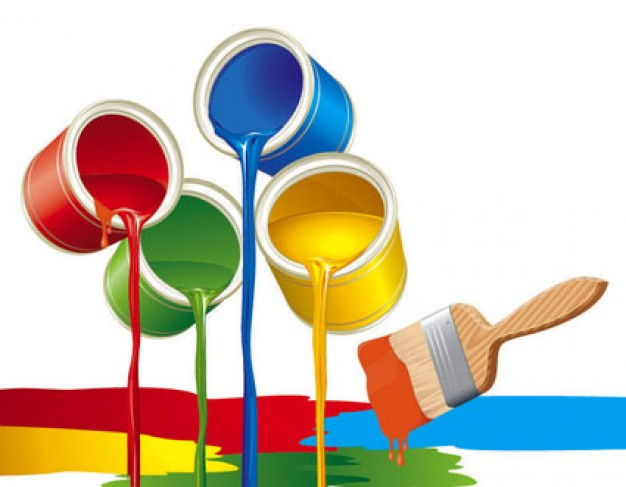
\includegraphics[scale=0.3]{figuras/desenho}
    }
    \fonte{o autor.}
\end{desenho}
\cleardoublepage

\section{CITAÇÃO}

Segundo  \citeonline[p. 94]{livro-unoesc},
\begin{citacao}
``Compreende trecho transcrito que apresenta mais de três linhas; mantém-se o discurso do texto original; destaca-se em blocos, espaço simples,com recuo de 4 cm a partir da margem esquerda, com letra menor que a do texto original;sugere-se usar tamanho 10''.
\end{citacao}

\section {LISTAS}
 Lorem ipsum dolor sit amet, consectetuer adipiscing elit. Ut purus elit, vestibulum ut, placerat ac, adipiscing vitae, felis. Curabitur dictum gravida mauris. Nam arcu libero, nonummy eget, consectetuer id, vulputate a, magna.

\begin{itemize}
\item Nam dui ligula, fringilla.
\item Nam dui ligula, fringilla.
\item Nam dui ligula, fringilla.
\end{itemize}

Lorem ipsum dolor sit amet, consectetuer adipiscing elit. Ut purus elit, vestibulum ut, placerat ac, adipiscing vitae, felis. Curabitur dictum gravida mauris. Nam arcu libero, nonummy eget, consectetuer id, vulputate a, magna.

\begin{enumerate}
 \item enumA
 \item enumB
\end{enumerate}



%RESULTADOS
\chapter{RESULTADOS E DISCUSSÕES}

\lipsum[1-1]



%CONCLUSÃO
\chapter{CONCLUSÃO}

\lipsum[1-1]

% ----------------------------------------------------------
% ELEMENTOS PÓS-TEXTUAIS
% ----------------------------------------------------------
\postextual

% ----------------------------------------------------------
% Referências bibliográficas
% ----------------------------------------------------------

\bibliography{referencias}

%Apêndices
\begin{apendicesenv}

\chapter{TÍTULO DO APÊNDICE A}

Arquivos confeccionados pelo autor do trabalho e que não se encaixam no texto.

 Ex: Deduções matemáticas, dimensionamentos extensos e algoritmos.

\end{apendicesenv}

%Anexos
\begin{anexosenv}
\chapter{Título do Anexo A}
\label{anexoA}

Arquivos não confeccionados pelo autor do trabalho.
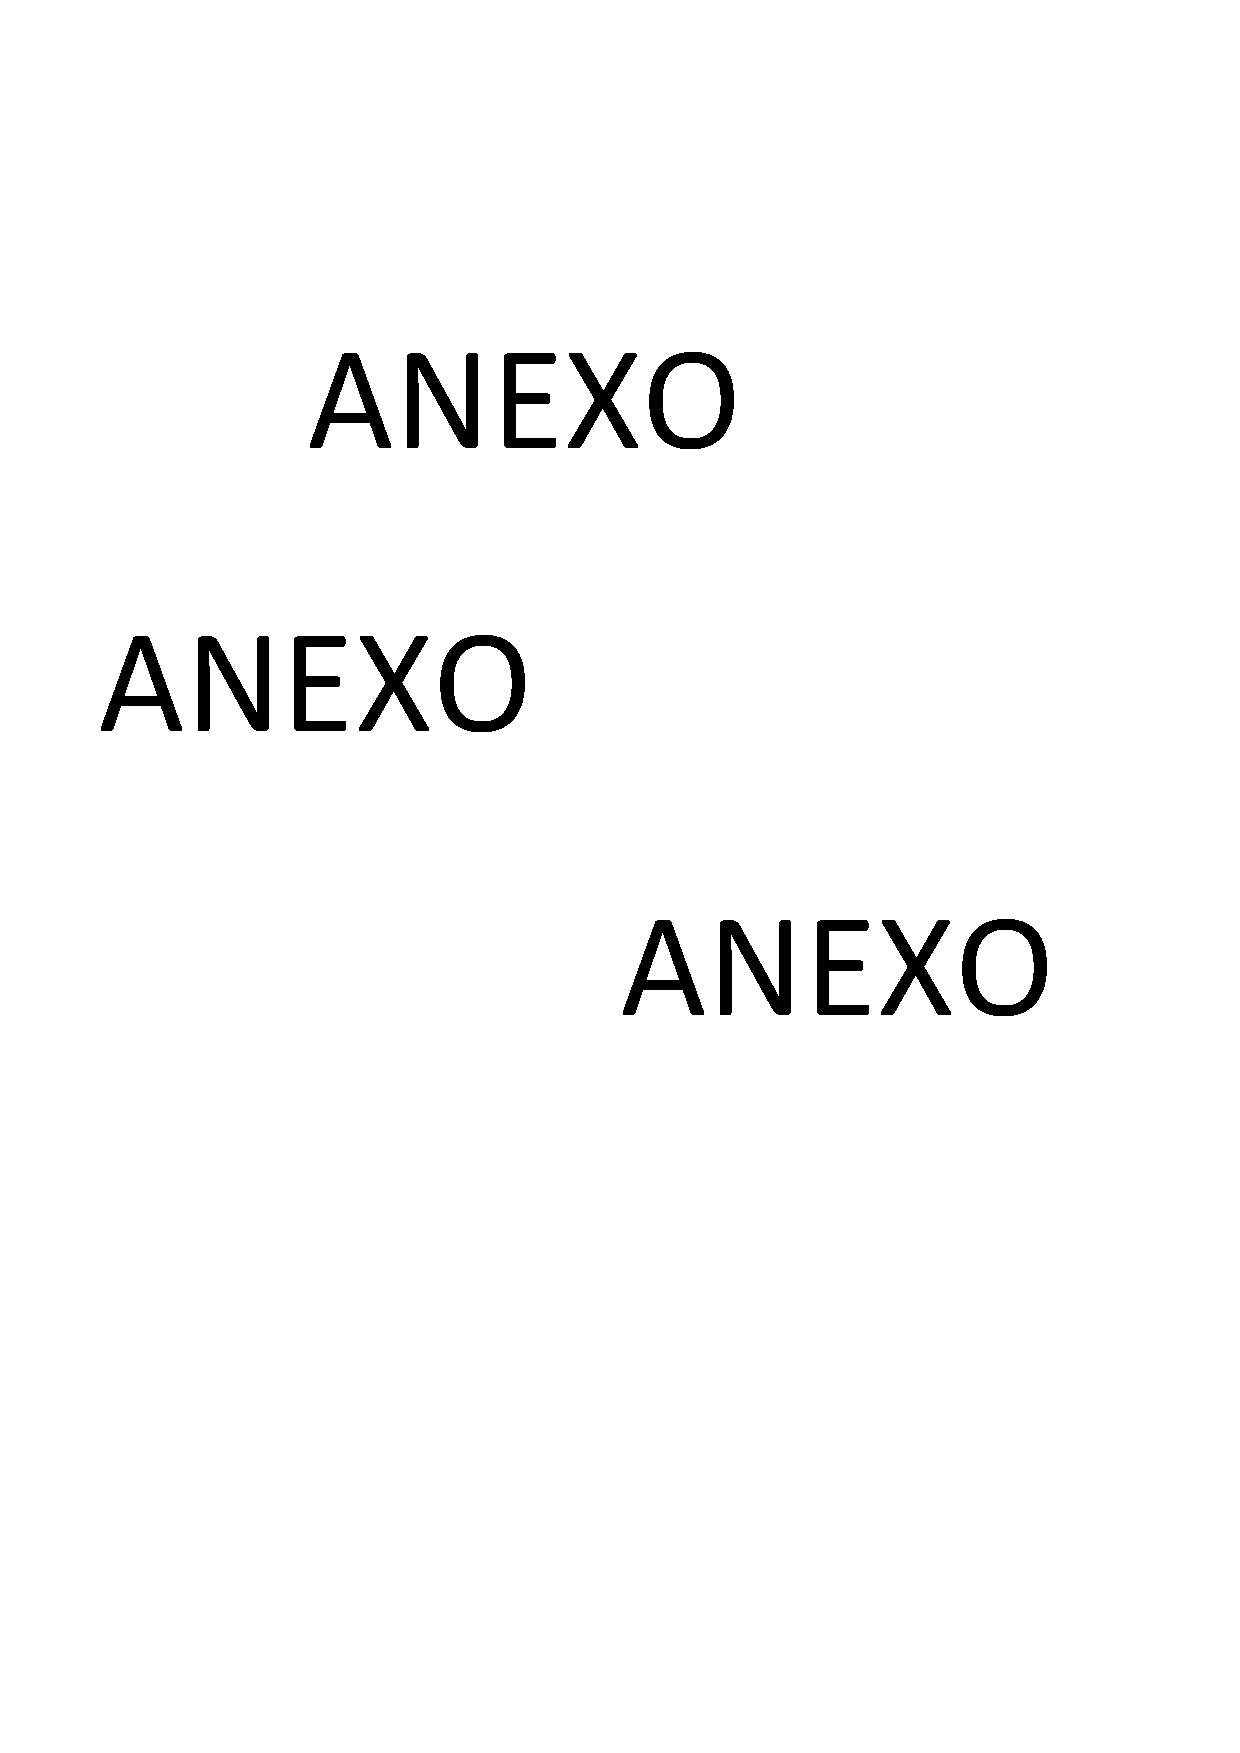
\includepdf{postextuais/anexo1}

\end{anexosenv}

%---------------------------------------------------------------------
% INDICE REMISSIVO
%---------------------------------------------------------------------

\printindex
\end{document}